\documentclass[10pt,a4paper]{article}
\usepackage[margin=2cm]{geometry}
\usepackage{amsmath,amssymb,bm}
\usepackage{booktabs,tabularx,multirow}
\usepackage{xcolor}
\usepackage{tikz}
\usetikzlibrary{arrows.meta,positioning,fit,backgrounds,calc,shapes.geometric}
\usepackage{pgfplots}
\pgfplotsset{compat=1.17}
\usepackage{microtype}
\usepackage{enumitem}
\usepackage{caption}
\usepackage[hidelinks]{hyperref}
\setlist{nosep,leftmargin=*}

\definecolor{recon}{HTML}{2E6FAC}
\definecolor{phys}{HTML}{C0504D}
\definecolor{robot}{HTML}{4F8A3C}
\definecolor{evalc}{HTML}{7F5FA8}
\definecolor{bad}{HTML}{C0504D}
\definecolor{good}{HTML}{4F8A3C}

\newcommand{\Log}{\operatorname{Log}}
\newcommand{\relu}{\operatorname{relu}}
\newcommand{\clip}{\operatorname{clip}}
\newcommand{\R}{\mathbb{R}}

\title{\textbf{From Egocentric Stereo Video to Robot-Hand Policies}\\[2pt]
\large NVIDIA V2D Challenge, Track 3 --- system review, formulation and results}
\author{Project log, Vulcan HPC (status 2026-10-01)}
\date{}

\begin{document}
\maketitle

\begin{abstract}
We reconstruct accurate, physically plausible 4D hands and objects from egocentric stereo video and use
them as references for training per-episode dexterous policies (floating Sharpa hands) in FlashCHORD
(Newton + MuJoCo-Warp, FlashSAC). The reconstruction fuses FoundationPose, stereo ICP and hand
evidence in a robust SE(3) trajectory optimisation with a cubic B-spline residual, contact-aware damping
and symmetry canonicalisation, followed by a stereo MANO hand fit, grasp plausibility (penetration, wrench
feasibility), an optional joint hand--object optimisation, a round-table model and a rest-settle step.
On the robot side we added a contact-location reward with an inside/outside gate. With it, all
eight single-object public episodes reach ADD-AUC $0.96$--$1.00$ (ep44: $0.49\to0.98$), and four of thirteen
two-object scenes exceed $0.79$. The remaining failures are concentrated in scenes with fine
object--object interaction (lid on pot, sweeper and dust pan, stacking).
\end{abstract}

\tableofcontents
\bigskip

%=====================================================================
\section{Task and data}
\begin{itemize}
\item \textbf{Input.} Egocentric rig: colour camera \texttt{ego\_cam\_a} (2028$\times$1520) plus a mono stereo pair
(1280$\times$800, 75\,mm baseline), recorded at \textbf{20\,fps} (20.25\,fps nominal). There are 20 public episodes, which have
mocap object poses but no hand ground truth, and 20 scored evaluation episodes, which are video only. The data covers
10 tasks and 10 scanned objects with meshes. A wooden spoon in 10 scored episodes has no public mesh.
\item \textbf{Output.} For each scored episode, train a policy, roll it out with the official
\texttt{evaluate\_policy.py}, and submit the object trajectory. The pose metrics are AUC, SP-SR, MP-SR, RPE and MPPE (Sec.~\ref{sec:metrics}).
A separate mesh file is scored by CD-O.
\item \textbf{Compute.} Everything runs as Slurm jobs (L40S 48\,GB) in Apptainer images converted from the
toolkit's Docker images. All data lives on \texttt{\$SCRATCH}.
\end{itemize}

%=====================================================================
\section{System overview}
Figure~\ref{fig:system} shows the full pipeline. Thick arrows connect whole groups: every perception output feeds the estimates, and all estimates feed the fusion. Blue boxes are perception and reconstruction,
red boxes enforce physical plausibility, green boxes are the robot-learning stage (NVIDIA's own code, with our
patches and reward), and purple boxes are evaluation.

\begin{figure}[h!]
\centering
\resizebox{\textwidth}{!}{%
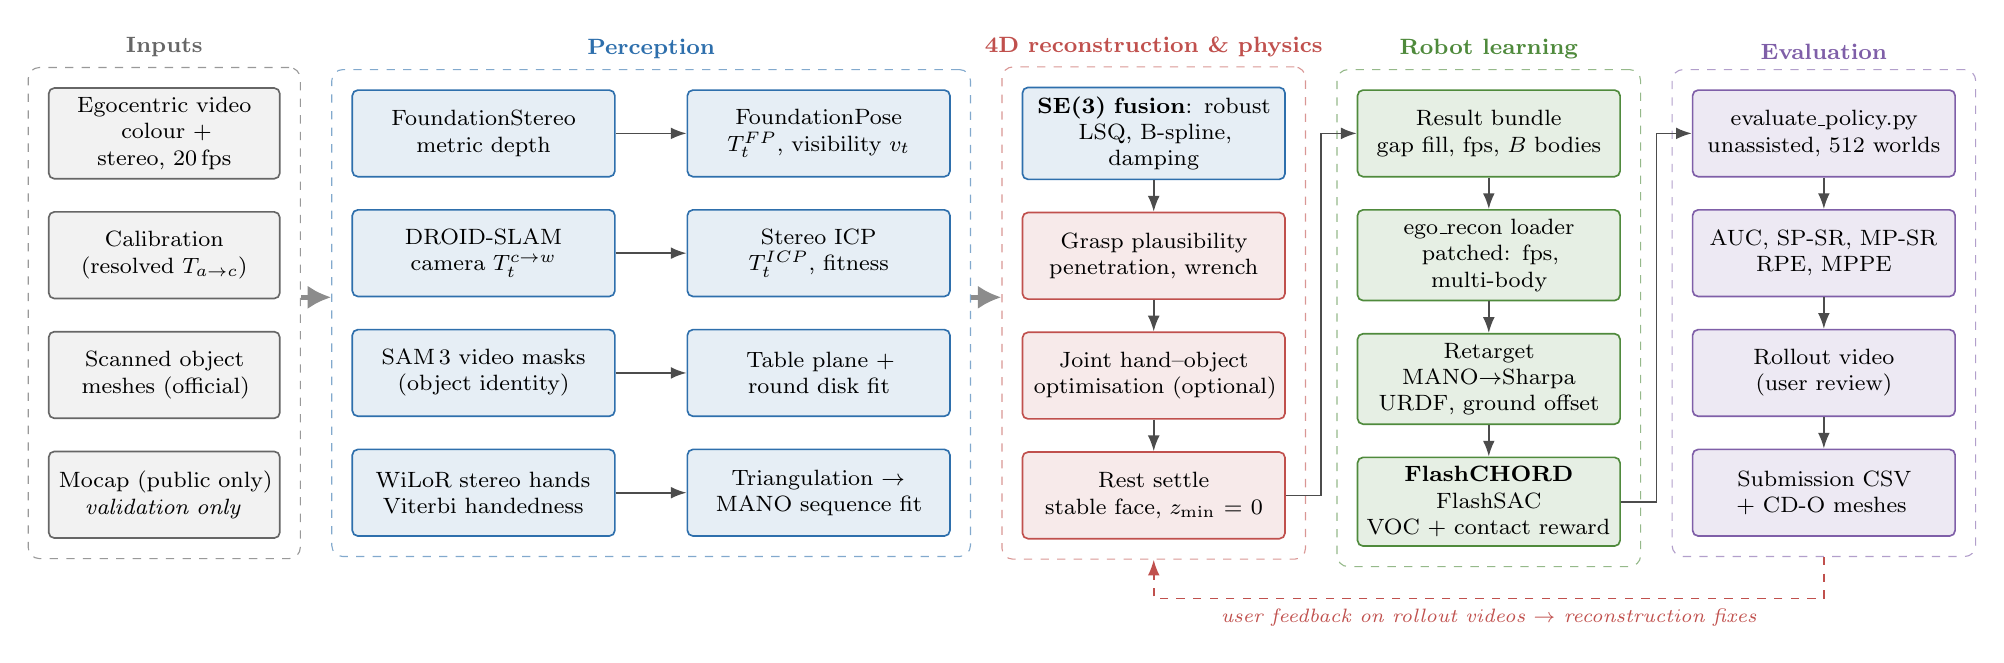
\begin{tikzpicture}[
  node distance=4mm and 9mm,
  box/.style={draw, rounded corners=2pt, minimum height=11mm, text width=31mm, align=center, font=\footnotesize, line width=0.6pt},
  rb/.style={box, fill=recon!12, draw=recon},
  pb/.style={box, fill=phys!12, draw=phys},
  gb/.style={box, fill=robot!14, draw=robot},
  eb/.style={box, fill=evalc!14, draw=evalc},
  io/.style={box, fill=black!5, draw=black!60, text width=27mm},
  ar/.style={-{Latex[length=2mm]}, line width=0.6pt, draw=black!70},
  big/.style={-{Latex[length=3mm,width=3mm]}, line width=1.6pt, draw=black!45},
  grp/.style={draw, dashed, rounded corners, inner sep=2.5mm},
  glab/.style={font=\footnotesize\bfseries, anchor=south}
]
% column 1: inputs
\node[io] (vid) {Egocentric video\\colour + stereo, 20\,fps};
\node[io, below=of vid] (calib) {Calibration\\(resolved $T_{a\to c}$)};
\node[io, below=of calib] (mesh) {Scanned object\\meshes (official)};
\node[io, below=of mesh] (dummy) {Mocap (public only)\\\emph{validation only}};
% column 2: perception
\node[rb, right=of vid] (depth) {FoundationStereo\\metric depth};
\node[rb, below=of depth] (slam) {DROID-SLAM\\camera $T^{c\to w}_t$};
\node[rb, below=of slam] (seg) {SAM\,3 video masks\\(object identity)};
\node[rb, below=of seg] (hands2d) {WiLoR stereo hands\\Viterbi handedness};
% column 3: estimates
\node[rb, right=of depth] (fp) {FoundationPose\\$T^{FP}_t$, visibility $v_t$};
\node[rb, below=of fp] (icp) {Stereo ICP\\$T^{ICP}_t$, fitness};
\node[rb, below=of icp] (table) {Table plane +\\round disk fit};
\node[rb, below=of table] (mano) {Triangulation $\to$\\MANO sequence fit};
% column 4: fusion & physics
\node[rb, right=of fp] (fuse) {\textbf{SE(3) fusion}: robust\\LSQ, B-spline, damping};
\node[pb, below=of fuse] (grasp) {Grasp plausibility\\penetration, wrench};
\node[pb, below=of grasp] (joint) {Joint hand--object\\optimisation (optional)};
\node[pb, below=of joint] (settle) {Rest settle\\stable face, $z_{\min}=0$};
% column 5: robot
\node[gb, right=of fuse] (export) {Result bundle\\gap fill, fps, $B$ bodies};
\node[gb, below=of export] (loader) {ego\_recon loader\\patched: fps, multi-body};
\node[gb, below=of loader] (retarget) {Retarget MANO$\to$Sharpa\\URDF, ground offset};
\node[gb, below=of retarget] (fc) {\textbf{FlashCHORD} FlashSAC\\VOC + contact reward};
% column 6: eval
\node[eb, right=of export] (evalp) {evaluate\_policy.py\\unassisted, 512 worlds};
\node[eb, below=of evalp] (metrics) {AUC, SP-SR, MP-SR\\RPE, MPPE};
\node[eb, below=of metrics] (video) {Rollout video\\(user review)};
\node[eb, below=of video] (sub) {Submission CSV\\+ CD-O meshes};

% groups
\node[grp, draw=black!40, fit=(vid)(dummy)] (G0) {};
\node[grp, draw=recon!60, fit=(depth)(hands2d)(fp)(mano)] (G1) {};
\node[grp, draw=phys!60, fit=(fuse)(settle)] (G2) {};
\node[grp, draw=robot!60, fit=(export)(fc)] (G3) {};
\node[grp, draw=evalc!60, fit=(evalp)(sub)] (G4) {};
\node[glab, text=black!60] at (G0.north) {Inputs};
\node[glab, text=recon] at (G1.north) {Perception};
\node[glab, text=phys] at (G2.north) {4D reconstruction \& physics};
\node[glab, text=robot] at (G3.north) {Robot learning};
\node[glab, text=evalc] at (G4.north) {Evaluation};

% row-wise perception -> estimates
\draw[ar] (depth) -- (fp);
\draw[ar] (slam) -- (icp);
\draw[ar] (seg) -- (table);
\draw[ar] (hands2d) -- (mano);
% inputs -> perception, estimates -> fusion (group level)
\draw[big] (G0.east |- slam.south) -- (G1.west |- slam.south);
\draw[big] (G1.east |- icp.south) -- (G2.west |- icp.south);
% chains
\foreach \x/\y in {fuse/grasp, grasp/joint, joint/settle, export/loader, loader/retarget, retarget/fc, evalp/metrics, metrics/video, video/sub}
  \draw[ar] (\x) -- (\y);
% chain to chain, through the column gaps
\draw[ar] (settle.east) -- ++(4.5mm,0) |- (export.west);
\draw[ar] (fc.east) -- ++(4.5mm,0) |- (evalp.west);
% feedback loop under the figure
\coordinate (low) at ($(G3.south)+(0,-4mm)$);
\draw[ar, dashed, draw=phys] (G4.south -| sub) -- (sub |- low) -- node[below, font=\scriptsize\itshape, text=phys]{user feedback on rollout videos $\to$ reconstruction fixes} (settle |- low) -- (G2.south -| settle);
\end{tikzpicture}}
\caption{System overview. Every stage runs as a Slurm job and writes a visualisation video for review. Mocap is used only to validate the reconstruction on public episodes, never as an input.}
\label{fig:system}
\end{figure}

%=====================================================================
\section{Perception}
\paragraph{Calibration.} The published \texttt{extrinsics\_to\_stereo\_left} of the colour camera actually
maps to the pre-relabel sensor \texttt{ego\_cam\_b}. Using $T_{a\to c}=T_{c\to b}^{-1}T$ reduces the
reprojection error from 18.9\,px to 3.4\,px. The stereo epipolar error is 1.9\,px.

\paragraph{Depth, camera and masks.} FoundationStereo provides metric depth and DROID-SLAM provides the camera
trajectory. SAM\,3 video masks replaced SAM\,2/GroundingDINO, whose masks were the main upstream failure mode (ep0, 18, 23, 24, 26, 31).

\paragraph{Hands.} Stereo WiLoR detections, with CLAHE and flipped-handedness passes, are associated by a Viterbi
handedness decoder and triangulated. The colour camera leads the stereo pair by about 0.65 frames, which is compensated.
A temporally smooth MANO sequence fit follows. It reaches about 6\,mm MPJPE to the triangulation, compared with about 24\,mm for HaWoR after wrist
alignment, and the user chose it in a visual comparison. Per-frame hand ``corrections'' were rejected
because they introduced jitter.

%=====================================================================
\section{Object trajectory fusion}
\subsection{Robust SE(3) least squares}
For each object the unknowns are per-frame poses $(R_t,p_t)$, with $R_t=\exp(\delta_t)R_t^0$. Each grasp
segment $k$ has a grasp offset $G_k=(R_G,t_G)$ relative to the hand, and each span has spline control points $c_j$
and $C_j$. We minimise
\begin{equation}
\min\;\tfrac12\sum_i \rho\!\left(f_i^2\right),\qquad \rho(s)=2\left(\sqrt{1+s}-1\right)\quad\text{(soft-}L_1\text{, per scalar residual)},
\end{equation}
with the residual blocks below (default scales in brackets):
\begin{align}
\text{measurement:}\;& \sqrt{w_t}\,\frac{p_t-p_m}{\sigma_t},\;\; \sqrt{w_r}\,\frac{\Log(R_m^\top R_t)}{\sigma_r}
 && [\sigma_t{=}1\,\text{cm},\ \sigma_r{=}5^\circ]\\
\text{acceleration:}\;& \frac{p_{t+1}-2p_t+p_{t-1}}{\sigma_{acc}},\;\; \frac{\omega_t-\omega_{t-1}}{\sigma_{racc}},\;\; \omega_t=\Log(R_t^\top R_{t+1})
 && [4\,\text{mm},\ 2^\circ]\\
\text{damping:}\;& \sqrt{s_t}\left[\frac{p_{t+1}-p_t}{\sigma_{vel}},\ \frac{\omega_t}{\sigma_{rvel}}\right]
 && [1\,\text{mm},\ 0.3^\circ]\\
\text{grasp:}\;& \sqrt{w}\left[\frac{p_t-H^R_t t_G-H^p_t}{\sigma_{gt}},\ \frac{\Log\!\big((H^R_tR_G)^\top R_t\big)}{\sigma_{gr}}\right]
 && [6\,\text{mm},\ 4^\circ]\\
\text{follow:}\;& \sqrt{w}\left[\frac{p_{t+1}-D_Rp_t-d}{\sigma_{ft}},\ \frac{\Log\!\big((D_RR_t)^\top R_{t+1}\big)}{\sigma_{fr}}\right],\; D=H_{t+1}H_t^{-1}
 && [4\,\text{mm},\ 3^\circ]\\
\text{anchor:}\;& \delta_t/\sigma_{anchor} && [60^\circ]
\end{align}
Here $H_t$ is the hand (palm) pose. Acceleration and velocity scales are rescaled with the frame rate, by $(20/f)^2$ and $(20/f)$.
Measurements come from FoundationPose, with $(w_t,w_r)=(v,v^2)$ and $v=\clip(A_t/P_{90}(A),0,1)$ the mask area relative to its 90th percentile,
and from stereo ICP, with $w=4\,\mathrm{fitness}^2$. ICP is kept only if fitness $\ge 0.5$, RMSE $\le 4$\,mm, there are at least 300 points and the jump is at most 5\,cm.
A residual is flagged as an outlier if $\|r/\sqrt w\|/\sqrt2>3$.

\subsection{Cubic B-spline residual}
Within each span (split at contact-phase changes and at gaps $>0.15$\,s) the trajectory is pulled toward a
cubic B-spline of itself. The control points are optimisation variables with clamped knots spaced $h=0.15$\,s:
\begin{equation}
\sqrt{w}\,\frac{p_t-\sum_j B_{tj}c_j}{\sigma_t},\qquad
\sqrt{w}\,\frac{\Log(S_t^\top R_t)}{\sigma_r},\qquad
S_t=C_b\prod_{q=1}^{3}\exp\!\Big(\tilde B_{t,b+q}\,\Log(C_{b+q-1}^\top C_{b+q})\Big),
\end{equation}
where $\tilde B_{tj}=\sum_{i\ge j}B_{ti}$ (cumulative SO(3) B-spline). A ridge term $\sqrt{w\lambda}\,Dc/\sigma_t$, with $\lambda=0.1$ and $D$
the second divided difference at the Greville abscissae, regularises the control polygon. The spline weight is $w=0.2$.
This replaced an earlier version that pulled the trajectory toward a \emph{pre-smoothed initial guess} (a pseudo-measurement bug).

\subsection{Damping, symmetry, contact phases}
\begin{itemize}
\item \textbf{Damping weight.} The weight is $s_t=\max(\mathrm{free}_t\,\mathrm{rest}_t,\ \mathrm{occl}_t,\ \mathrm{still}_t)$. Only the
``free'' (no hand nearby) part is gated by
$\mathrm{rest}_t=\mathrm{sup}_t\,\mathrm{sup}_{t+1}\exp(-(\tilde v/0.04)^2-(\tilde\omega/0.5)^2)$. Earlier,
\texttt{static\_w *= rest} also removed the occlusion and still-hand damping, which was a bug.
The other terms are $\mathrm{occl}_t=(1-\min(v_t,v_{t+1}))\mathbf 1[\neg\mathrm{held}]$ and $\mathrm{still}=\exp(-(\bar v_{palm}/4\,\mathrm{mm})^2)$.
\item \textbf{Symmetry.} Symmetry groups are detected by ADD-S self-distance below 5\,mm, giving either a continuous axis or discrete $180^\circ$ flips.
All sources are canonicalised in one merged, time-ordered pass with $g^*=\arg\max_g\operatorname{tr}(R_{ref}^\top R_m g)$, keeping the centroid fixed:
$R'=Rg^*$ and $p'=p+R(c-g^*c)$.
\item \textbf{Contact phases.} A hand side touches the object if at least 2 confident joints are within 2.5\,cm of the object surface. Phase runs shorter than 3 frames are debounced into
their longer neighbour. A grasp segment is a single-side run of at least 4 frames.
\end{itemize}
Over the 22 objects with ICP coverage, fusion gives 0.98\,cm mean error against mocap, compared with 1.05\,cm for FoundationPose alone. Frame-to-frame jitter
drops from 1.74\,mm to 0.74\,mm.

%=====================================================================
\section{Physical plausibility}
\subsection{Round table model}
The table is fitted as a plane (RANSAC with $|x\cdot n-h|<8$\,mm, refined by SVD; it matches the mocap vertical to 1--3$^\circ$). It is then fitted as a
\textbf{disk}: a circle fitted by RANSAC to the occupancy-grid contour, followed by Kåsa refinement,
$[2x\;2y\;1][c_x\;c_y\;k]^\top=x^2+y^2$ with $r=\sqrt{k+\|c\|^2}$ (about 0.24--0.29\,m), and a nominal slab thickness $\tau=3$\,cm.
Hands may legitimately pass below the table outside the disk. The penetration depth of a point is, with $d=x-c$,
$h=d\cdot u$, $r=\|d-hu\|$ and the soft inside test $\iota=\clip\big((R+s-r)/2s,0,1\big)$:
\begin{equation}
\mathrm{depth}(x)=\begin{cases}\iota\,\relu(-h) & \text{body mostly above the table } (\bar h>-\tau/2)\\[2pt]
\iota\,\relu(h+\tau)\,\mathbf 1[-\tau<h<0] & \text{body below (pushed out through the underside)}\end{cases}
\end{equation}
The \texttt{side="auto"} rule fixed a bug in which the nearest face pushed bodies through the slab.

\subsection{Grasp plausibility and wrench feasibility}
Hand candidates are smooth, knot-based corrections of the MANO fit, with contacts anchored in the object frame and squeezes of 1.5, 3 and 5\,mm.
Each is tested for penetration (pass if P95 $\le$ 5\,mm and fewer than 5\% of frames exceed 10\,mm) and for \emph{wrench feasibility}. The required object wrench is
\begin{equation}
F=m(a+g\,u),\qquad \tau=I_w\alpha+\omega\times I_w\omega,\qquad I_w=RIR^\top .
\end{equation}
Contacts are hand vertices with $|\mathrm{sdf}|<5$\,mm, merged into 1\,cm patches, and each patch's friction cone is
linearised with 8 edges, $e_{ck}=\mathrm{normalize}\big(n_c+\mu(\cos\theta_k t_1+\sin\theta_k t_2)\big)$.
A frame is feasible if
\begin{equation}
r=\frac{\min_{\lambda\ge0}\|A\lambda-b\|}{\|b\|}<0.1,\qquad A_{:,ck}=\begin{bmatrix}e_{ck}\\ (p_c-c)\times e_{ck}/0.1\end{bmatrix},\quad b=\begin{bmatrix}F\\ \tau/0.1\end{bmatrix},
\end{equation}
which is solved by NNLS at $\mu\in\{0.1,1.0\}$. With $\mu=1$, 80--100\% of lifted frames are feasible after correction, and penetration drops from 7--24\,mm to 1--4\,mm.

\subsection{Joint hand--object optimisation}
This stage jointly refines object poses, grasp offsets with bounded slip, and hands in the world frame, using Adam (300 iterations on objects and $G$, then 900 on everything).
Object keypoints are $K_{tk}=c_t+R_td_k$ with $d_k\in\{0,\pm5\,\text{cm}\,e_{x,y,z}\}$. Corrections are bounded by
$\mathrm{bnd}_L(x)=Lx/\sqrt{1+\|x\|^2}$ (object 40\,mm and $25^\circ$; grasp offset 30\,mm and $25^\circ$; slip 10\,mm and $8^\circ$).
\begin{multline}
\mathcal L=10^4\mathcal L_{obs}+3{\cdot}10^4\mathcal L_{couple}+10^5\mathcal L_{slip}+4{\cdot}10^6\mathcal L_{slip\text{-}vel}
+10^6(\mathcal L_{static}+\mathcal L_{nohand})+400\,\mathcal L_{prior}\\
+6{\cdot}10^4\mathcal L_{acc}+6{\cdot}10^3\mathcal L_{spline}+2{\cdot}10^4(\mathcal L_{table}+\mathcal L_{pen})
+3{\cdot}10^3\mathcal L_{anchor}+1.5{\cdot}10^3\mathcal L_{data}+10^3\mathcal L_{tri}+\dots
\end{multline}
The coupling term ties the object to the hand during grasps ($s_g=15$\,mm):
\begin{equation}
\mathcal L_{couple}=\sum w_t\, s_g^2\,\rho\Big(\overline{\big\|K_{tk}-\big(H^R_tR_G(c+d_k)+H^R_tt_G+H^p_t\big)\big\|^2}\,/\,s_g^2\Big).
\end{equation}
\emph{Finding:} this helps hand-carried cups but hurts the pitcher and the beige cup, and it lowers the official AUC slightly. It is optional.

\subsection{Rest settle (new)}
\label{sec:settle}
In the table frame ($z=0$ is the top), a rest segment is a run of at least 5 frames in which the object is static ($v<2$\,cm/s, $\omega<15^\circ$/s), low
($|z_{\min}|<15$\,mm) and over the disk. For each convex-hull face $f$, the COM margin is
$m_f=-\max_i(a_i\cdot c_{2D}+b_i)$, where the half-planes $(a_i,b_i)$ bound the face's support polygon. Among faces with $m_f\ge0.3$\,mm and
$\angle(f,\hat d)\le8^\circ$, where $\hat d$ is the mean table normal in the object frame, the nearest face with $m_f\ge3$\,mm is chosen, or else the one with the largest margin.
Each frame is then rotated minimally about its COM so that $R_tf\to-e_z$, and lifted so that $z_{\min}=0$:
\begin{equation}
R'_t=\Delta_tR_t,\qquad p'_t=c_t-R'_t\,\mathrm{com}+\delta z_t\,e_z,\qquad \delta z_t=-\min_v\big(R'_tv+c_t-R'_t\mathrm{com}\big)_z .
\end{equation}
The correction is bridged across gaps of up to 8 frames and ramped out over 4 frames. It uses no mocap.

%=====================================================================
\section{Bridge to the robot pipeline}
\begin{itemize}
\item \textbf{Frame rate bug.} NVIDIA's loader hard-codes 30\,fps, but the videos are 20\,fps, so references played 1.5$\times$ too fast. We now read the fps from the
bundle, and the patched loader is bind-mounted into the image so the patch actually takes effect.
\item \textbf{Hands.} Gaps are filled in the world frame (interior gaps by lerp/slerp, leading and trailing gaps held), because the loader ignores
\texttt{is\_valid}: a zero hand would otherwise appear at the camera.
\item \textbf{Multi-object.} One rigid URDF per body, with slot order taken from the official evaluation list or the episode parquet.
\item \textbf{Ground offset (new).} The loader moved the scene so that the lowest frame-0 object point sat at $z=0$, about 4\,mm off our table in ep18. We now pass
\texttt{--ground\_z\_offset}, so the simulator ground is our table top.
\end{itemize}

%=====================================================================
\section{Robot learning}
\subsection{FlashCHORD setup}
The policy is learned with FlashSAC on floating Sharpa hands for 250M environment steps, with 2048 worlds (\texttt{njmax}=1024, \texttt{nconmax}=512; 4096 worlds run out of memory).
Contact friction is $\mu=1$ on all shapes, and objects use CoACD convex decomposition. The \textbf{VOC assist} applies a virtual wrench that pulls the object toward
the reference:
\begin{equation}
F=\clip_{200\,\mathrm N}\!\Big(s\big[m(400(p^*-p)-40v)+mg\,e_z\big]\Big),\qquad
\tau=\clip_{50\,\mathrm{Nm}}\!\Big(s\,\bar I\big[400\Log(q^*q^{-1})-40\omega\big]\Big).
\end{equation}
Its scale $s$ steps down through $1,0.75,0.5,0.25,0.1,0.05,0.025,0.01,0$ at about 19.7M, 34.4M, \dots, 122.9M steps. From 200M steps, half of the resets start
at the first frame.

\subsection{Reward}
The reward is $r_t=\Delta t\sum_i w_iT_i$, with the Laplacian shaping $\exp(-\sqrt{\mathrm{sse}}/\mathrm{var})$. The canonical terms are:
\begin{align}
T_{obj}&=\tfrac1{6B}\textstyle\sum_{b,k}\exp\!\big(-\|x^{sim}_{bk}-x^{ref}_{bk}\|/0.1\big),\quad x=p+Re_k \hspace{2em}(w=20)\\
T_{hand}&=\tfrac1H\textstyle\sum_h\tfrac1K\sum_k\exp(-\|x-x^*\|/0.1)\;(w=0.25),\qquad T_{q}=\tfrac1H\sum_h\exp(-\|q_h-q_h^*\|)\;(w=0.25)\\
s_k&=\max\!\big(0,\max_{c,e}d_k\cdot[f_{ce};\,p_c\times f_{ce}/r_c]\big),\quad
\ell_k=\relu\big((1-\tau)s_k^*-s_k\big)^2+\relu\big(s_k-(1+\tau)s_k^*\big)^2\\
T_{wrench}&=\operatorname{mean}_{h,b}\tfrac1{|K^*|}\textstyle\sum_{k\in K^*}e^{-\ell_k/0.1}\quad(w=10),
\end{align}
plus missed contact ($-1$), unintended contact ($-10$), termination ($-100$, triggered by wrist error $>15$\,cm or object error $>10$\,cm / 0.5\,rad) and action
penalties ($-0.002$, $-0.005$). The wrench term uses 512 random wrench directions $d_k$ with a $\mu=0.1$ cone.
It is \emph{location-agnostic}: two grasps with the same wrench space score equally, which produced
the ``grasps the wrong part'' behaviour (dust-pan handle).

\paragraph{Our contact-location term.} The human contact targets $c$ and their outward normals $n$ are expressed in the object frame. For each robot
link at $p$ with half-thickness $r_l$,
\begin{equation}
T_{loc}=\frac1{N_h}\sum_l \exp\!\Big(-\frac{\max(\|p-c\|-r_l,0)}{0.02}\Big)\;\sigma\!\Big(\frac{(p-c)\cdot n}{0.003}\Big)\qquad(w=5),
\end{equation}
where the sigmoid separates the \emph{inside} and \emph{outside} surfaces of hollow objects (cups, pots). It is paired with
a touch term, $\mathbf 1[\text{sim contact},\|x_c-c\|<1.5\,\text{cm}]\,e^{-\|x_c-c\|/0.02}$ ($w=2$), and an unintended-location penalty ($w=-1$).
Contact targets come from semantic MANO slots, with hysteresis, gap filling and a 5-frame moving average.

\paragraph{Ablation (ep41, pot).} We also implemented action jitter/smoothness, wrist acceleration, object orientation and velocity,
task completion (200, given once at frame $T-2$) and progress terms. Table~\ref{tab:abl} shows that only the contact term is safe.

\begin{table}[!htb]
\centering\small
\begin{tabular}{lc}
\toprule
Reward variant (ep41) & ADD-AUC \\
\midrule
Canonical FlashCHORD & 0.979 \\
+ contact location (\textbf{chosen}) & 0.972 \\
+ object orientation/velocity (weaker object keypoints) & 0.92 \\
+ smoothness terms & 0.70 \\
Full V2D reward (all terms) & 0.22 \\
\bottomrule
\end{tabular}
\caption{Reward ablation. The smoothness and task-completion terms let the policy trade tracking for stillness.}
\label{tab:abl}
\end{table}

%=====================================================================
\section{Evaluation metrics}
\label{sec:metrics}
For each world, a single rigid transform aligns the first pose of object slot~0 to the reference: $q_A=q^{ref}_{0,0}\otimes(q^{ach}_{0,0})^*$ and
$o=p^{ref}_{0,0}-R_Ap^{ach}_{0,0}$. It is applied to all frames and all bodies, so the first-frame pose matters a great deal.
\begin{align}
\mathrm{ADD}_{tb}&=\tfrac1V\textstyle\sum_v\|(R_a-R_r)x_v+p_a-p_r\|\\
\mathrm{AUC}&=\tfrac18\big[\tfrac12f_1+f_2+\dots+f_8+\tfrac12f_9\big],\; f_\tau=\operatorname{mean}\mathbf 1[\mathrm{ADD}<\tau\,\mathrm{cm}]\\
\text{SP-SR}&:\ \operatorname{mean}_b\bar e^p_b\le10\,\text{cm}\ \wedge\ \operatorname{mean}_b\bar e^\theta_b\le0.5\,\text{rad}\\
\text{MP-SR}&:\ \forall b:\ \bar e^p_b<3\,\text{cm}\wedge\bar e^\theta_b<30^\circ\\
\mathrm{RPE}&=100\operatorname{mean}_{i<j}\big\|R_{a,i}^\top(p_{a,j}-p_{a,i})-R_{r,i}^\top(p_{r,j}-p_{r,i})\big\|\\
\mathrm{MPPE}&=100\operatorname{mean}_k\|(p_a+0.05R_ae_k)-(p_r+0.05R_re_k)\|
\end{align}
Locally we report the evaluator's ADD-AUC, CHORD success rate and ManipTrans success rate, unassisted over 512 worlds.

%=====================================================================
\section{Results}
\subsection{Single-object public episodes (final checkpoint, 250M steps)}
\begin{table}[!htb]
\centering\small
\begin{tabular}{lcccc}
\toprule
Episode & Canonical reward & Contact reward & SR (contact) & Note\\
\midrule
ep12 (blue cup) & 0.728 & \textbf{0.984} & 100\% & ManipTrans SR 18\%$\to$100\%\\
ep39 (dust pan, handover) & 0.19$^\dagger$ & \textbf{0.961} & 98\% & real two-hand handover\\
ep40 & 0.983 & \textbf{0.992} & & \\
ep41 (pot) & \textbf{0.979} & 0.972 & 100\% & \\
ep42 & 0.993 & 0.993 & & \\
ep43 & 0.955 & 0.957 & & \\
ep44 (pot) & 0.489 & \textbf{0.976} & & largest gain\\
ep45 & 0.997 & 0.996 & & \\
\bottomrule
\end{tabular}
\caption{ADD-AUC, unassisted. $^\dagger$ on older reconstruction data. These parquets were converted at 30\,fps, before the fps fix.}
\end{table}

\clearpage
\subsection{Two-object public episodes (contact reward)}
\begin{figure}[!htb]
\centering
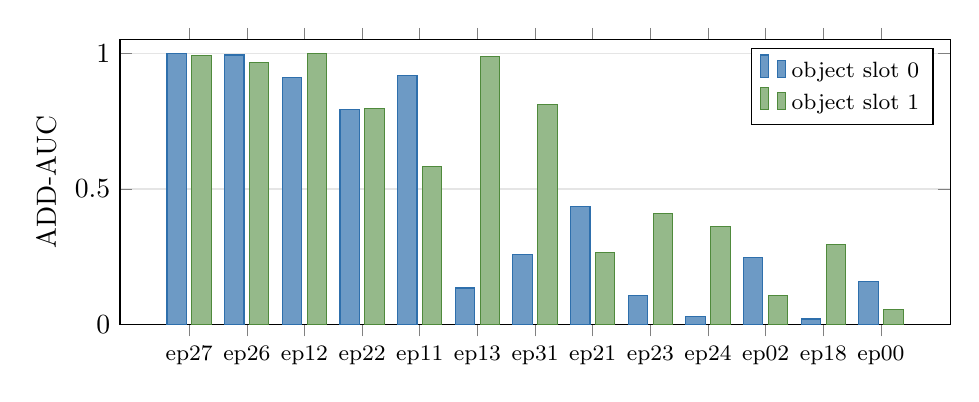
\begin{tikzpicture}
\begin{axis}[
  ybar, bar width=7pt, width=\textwidth, height=5.2cm,
  ymin=0, ymax=1.05, ylabel={ADD-AUC},
  symbolic x coords={ep27,ep26,ep12,ep22,ep11,ep13,ep31,ep21,ep23,ep24,ep02,ep18,ep00},
  xtick=data, x tick label style={font=\footnotesize},
  legend style={at={(0.98,0.97)}, anchor=north east, font=\footnotesize},
  ymajorgrids, grid style={black!10}]
\addplot[fill=recon!70, draw=recon] coordinates {(ep27,1.000)(ep26,0.994)(ep12,0.912)(ep22,0.793)(ep11,0.919)(ep13,0.135)(ep31,0.260)(ep21,0.437)(ep23,0.108)(ep24,0.029)(ep02,0.247)(ep18,0.021)(ep00,0.158)};
\addplot[fill=robot!60, draw=robot] coordinates {(ep27,0.991)(ep26,0.966)(ep12,1.000)(ep22,0.796)(ep11,0.582)(ep13,0.988)(ep31,0.811)(ep21,0.265)(ep23,0.410)(ep24,0.363)(ep02,0.107)(ep18,0.294)(ep00,0.056)};
\legend{object slot 0, object slot 1}
\end{axis}
\end{tikzpicture}
\caption{Per-object ADD-AUC for the 13 two-object scenes, sorted by the episode mean.}
\end{figure}

\begin{table}[!htb]
\centering\small
\begin{tabular}{llcccc}
\toprule
Ep. & Objects & AUC & CHORD SR & ManipTrans SR & Pos.\ err.\\
\midrule
27 & dish rack + pot & \textcolor{good}{0.995} & 100\% & 100\% & 0.5\,cm\\
26 & dish rack + pot & \textcolor{good}{0.980} & 100\% & 100\% & 0.7\,cm\\
12 & cup + dish rack & \textcolor{good}{0.956} & 99\% & 99\% & 0.8\,cm\\
22 & cup + pitcher & \textcolor{good}{0.795} & 91\% & 91\% & 2.7\,cm\\
11 & blue + beige cup & 0.751 & 99\% & 0\% & 2.8\,cm\\
13 & cup + dish rack & 0.561 & 0\% & 0\% & 8.4\,cm\\
31 & sweeper + dish rack & 0.535 & 75\% & 0\% & 4.7\,cm\\
21 & cup + pitcher & 0.351 & 0\% & 0\% & 10.5\,cm\\
23 & wooden pieces & \textcolor{bad}{0.259} & 0\% & 0\% & 12.4\,cm\\
24 & wooden pieces & \textcolor{bad}{0.196} & 0\% & 0\% & 12.0\,cm\\
02 & pot + lid & \textcolor{bad}{0.177} & 0\% & 0\% & 11.3\,cm\\
18 & sweeper + dust pan & \textcolor{bad}{0.158} & 0\% & 0\% & 8.5\,cm\\
00 & pot + lid & \textcolor{bad}{0.107} & 0\% & 0\% & 12.4\,cm\\
\bottomrule
\end{tabular}
\caption{Two-object scenes. Every world in the failing scenes terminates on the object criterion, and their orientation errors are 50--90$^\circ$.
With rest settle and the ground offset, ep18 reaches 0.189: the sweeper is still wrong from the first frame, so the cause is open.}
\end{table}

%=====================================================================
\section{Lessons learned}
\begin{enumerate}
\item \textbf{Timing matters before anything else.} The 30 vs 20\,fps mismatch silently made every reference 1.5$\times$ too fast. Stereo, colour and mocap
also lag each other by 0.3--1.4 frames.
\item \textbf{Segmentation was the bottleneck} of object tracking. SAM\,3 fixed most failures.
\item \textbf{Smooth, small corrections only.} Per-frame hand or object corrections create jitter. Spline-parameterised corrections do not.
\item \textbf{Location-agnostic rewards produce wrong grasps.} A contact-location term with an inside/outside gate fixed this, and smoothness and completion terms hurt.
\item \textbf{Physics punishes millimetre errors.} The sweeper's 1--5$^\circ$ tilt and 4--9\,mm table penetration are invisible in video, but
they put its centre of mass outside its support polygon. The scanned rounded base gives only a 0.9\,mm margin.
\item \textbf{Tests that pass are not proof.} Two fixes (carry-trim, ICP retime) passed synthetic tests and were then disabled because they were a net loss on real episodes.
\end{enumerate}

\section{Open problems and next steps}
\begin{itemize}
\item Two-object failures: check the references for object--object penetration, lid symmetry flips and infeasible second-object contacts. Test
lower object friction ($\mu=0.4$ for objects, 1.0 for the hand).
\item ep18: the sweeper is wrong from frame~0 even after settling. Inspect the first frame in the simulator. A compliant (flat) collision base
would be a simulation-asset change and needs a check against the rules first.
\item The early pitcher lift (ep22) comes from a noisy stereo palm in the grasp term. The proposed fix is a grasp that follows the MANO wrist, with agreement gating.
\item Scored episodes: MANO fits, the full pipeline and multi-object conversion are still needed. The wooden spoon needs a reconstructed mesh.
\item Re-convert the single-object episodes at 20\,fps, map evaluation steps to dataset frames, and pack the submission.
\end{itemize}

\end{document}
